
\begin{figure}


    \centering
    
    \hspace{2em}
    \textbf{MATLAB}\hspace{10em}
    \textbf{Python with modification}
    
    \hspace{-2em}
    
\includegraphics[trim=3cm 4cm 3cm 4cm, clip=true, height=.25\linewidth]{Figures/Fig_T5/MATLAB/ST_T2_Seg3_Var_Trajectory.eps}
    \hspace{4em}
    
\includegraphics[trim=6.5cm 4.5cm 6cm 4.5cm, clip=true,  height=.25\linewidth]{Figures/Fig_T5/ImprovP/ST_T2_Seg3_Var_Trajectory.eps} \\
    

    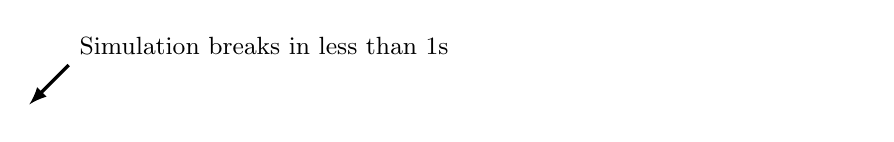
\begin{tikzpicture}  \node (image) at (0,0) {
    };
    \draw[latex-, very thick,black] (-10.5,0)  -- (-10,0.5)
        node[anchor=south west,black,fill=white]{\small Simulation breaks in less than 1s};
        
    \end{tikzpicture}
    \textbf{\rotatebox{90}{$\theta_1$}}\begin{subfigure}{\textwidth}
        \centering

        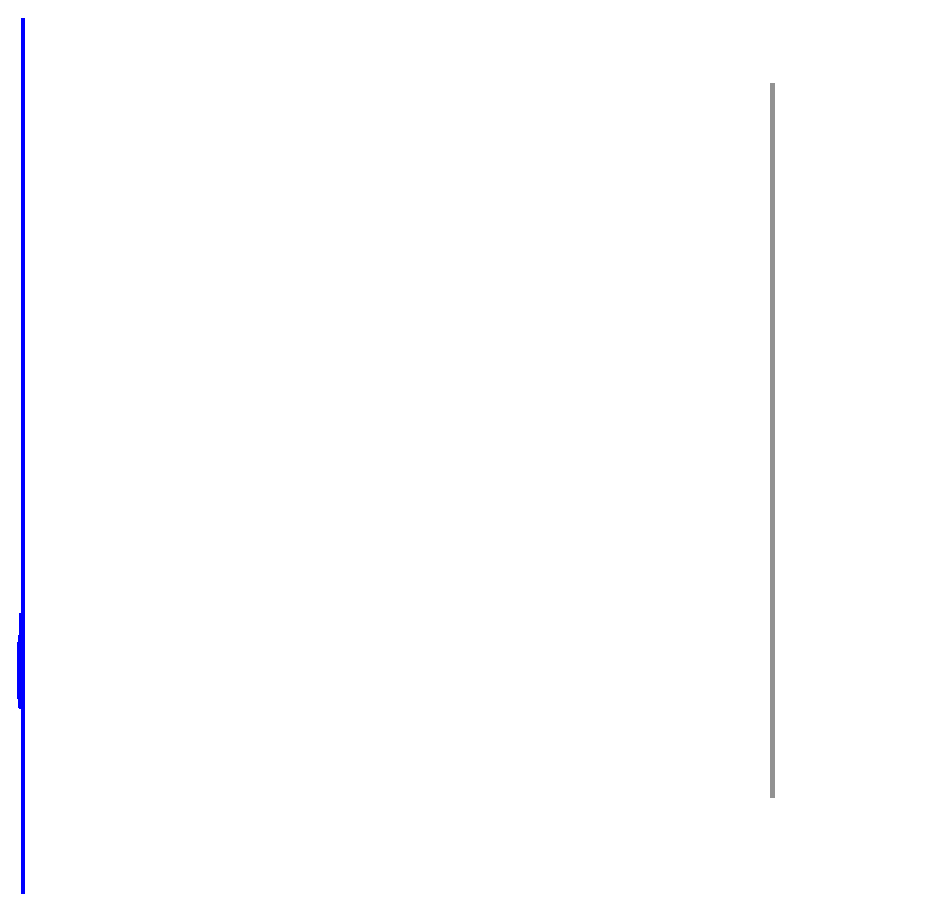
\includegraphics[trim=0cm 0cm 0cm 0cm,clip=true,height=0.1\linewidth,width=.45\linewidth]{Figures/Fig_T5/MATLAB/ST_T2_Seg3_Var_Theta0.eps}
        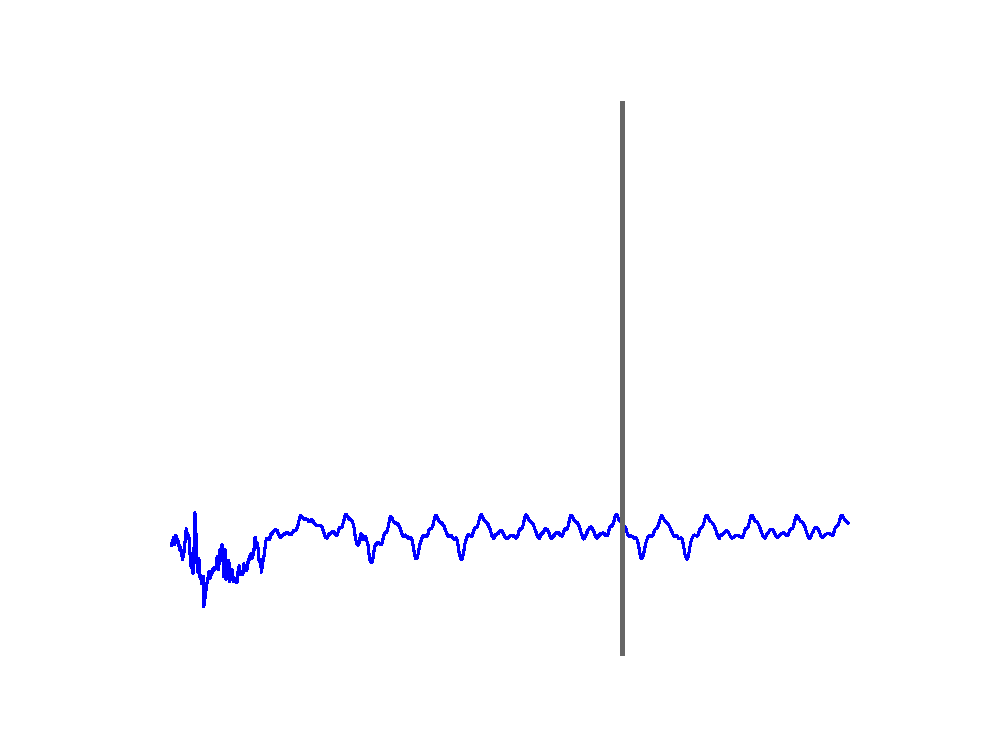
\includegraphics[trim=2cm 1cm 2cm 1cm,clip=true,height=0.1\linewidth,width=.45\linewidth]{Figures/Fig_T5/ImprovP/ST_T2_Seg3_Var_Theta0.eps}

    \end{subfigure}
    
        
        
    \textbf{\rotatebox{90}{$\theta_2$}}\begin{subfigure}{\textwidth}
        \centering
        
        \includegraphics[trim=0cm 0cm 0cm 0cm,clip=true,height=0.1\linewidth,width=.45\linewidth]{Figures/Fig_T5/MATLAB/ST_T2_Seg3_Var_Theta1.eps}
        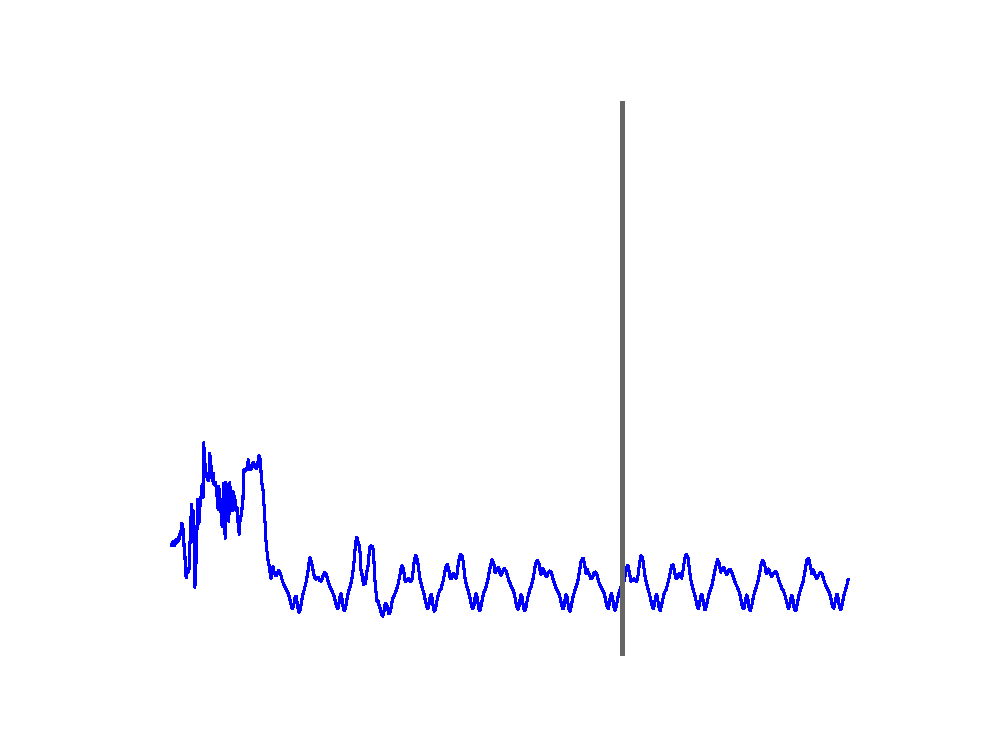
\includegraphics[trim=2cm 1cm 2cm 1cm,clip=true,height=0.1\linewidth,width=.45\linewidth]{Figures/Fig_T5/ImprovP/ST_T2_Seg3_Var_Theta1.eps}   

    \end{subfigure}
    
    
    \textbf{\rotatebox{90}{$\theta_3$}}\begin{subfigure}{\textwidth}
        \centering
        
        
\includegraphics[trim=0cm 0cm 0cm 0cm,clip=true,height=0.1\linewidth,width=.45\linewidth]{Figures/Fig_T5/MATLAB/ST_T2_Seg3_Var_Theta2.eps}
        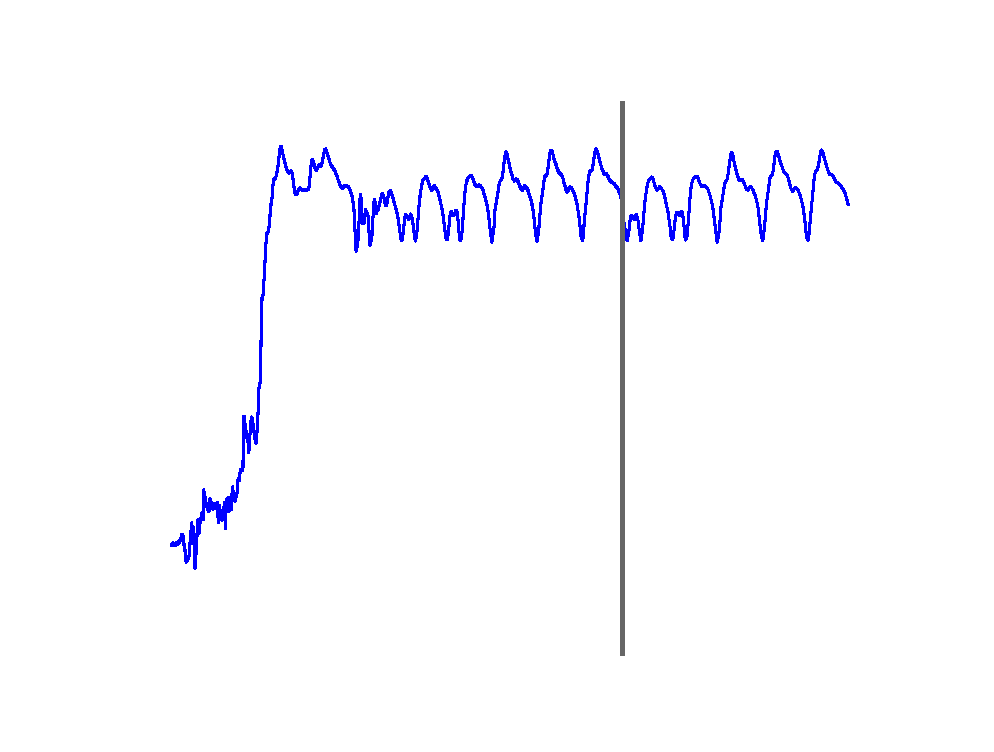
\includegraphics[trim=2cm 1cm 2cm 1cm,clip=true,height=0.1\linewidth,width=.45\linewidth]{Figures/Fig_T5/ImprovP/ST_T2_Seg3_Var_Theta2.eps}  
    
    \end{subfigure}
    
    \vspace{4em}
    
    \textbf{\rotatebox{90}{$||W||$}}\begin{subfigure}{\textwidth}
        \centering
        
        \hspace{.5em}
        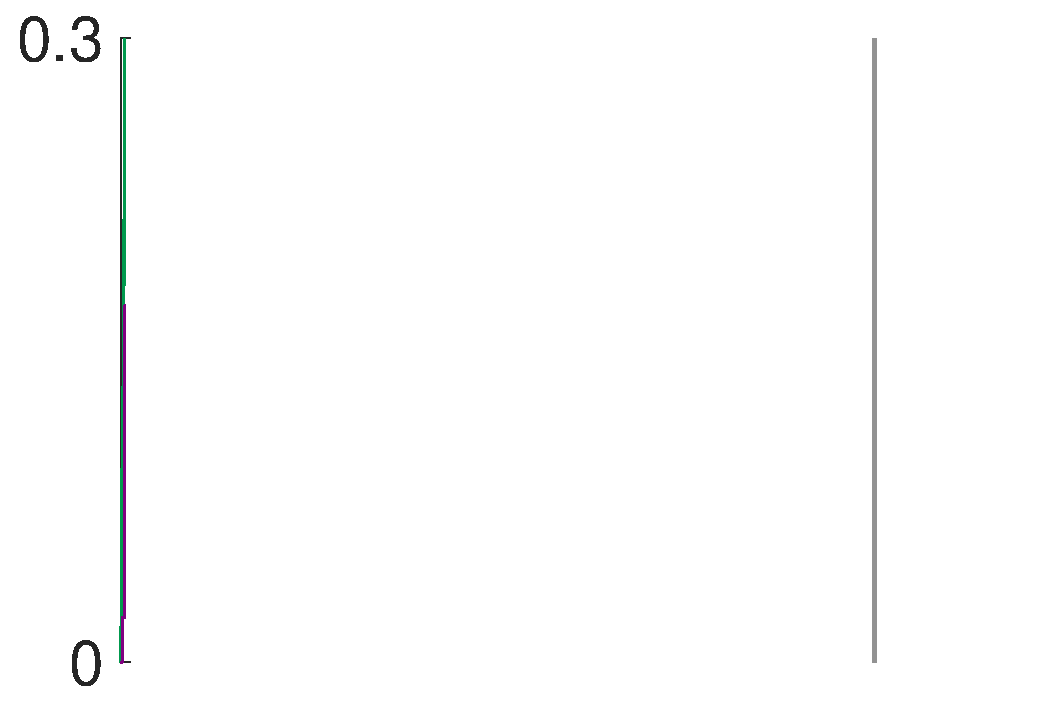
\includegraphics[trim=0cm 0cm 0cm 0cm,clip=true,height=0.15\linewidth,width=.45\linewidth]{Figures/Fig_T5/MATLAB/ST_T2_Seg3_Var_W_norm.eps}
        \hspace{0em}
        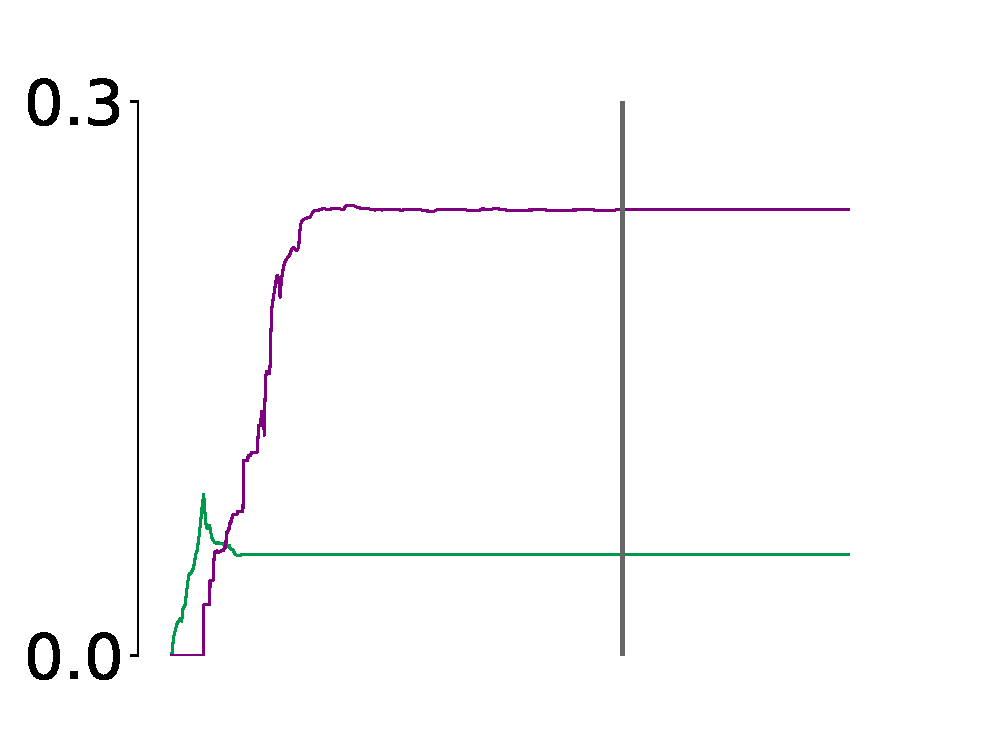
\includegraphics[trim=0cm 0cm 0cm 0cm,clip=true,height=0.15\linewidth,width=.45\linewidth]{Figures/Fig_T5/ImprovP/ST_T2_Seg3_Var_W_norm.eps}
    
    \end{subfigure}
    
    
    \vspace{4em}
    
    \textbf{\rotatebox{90}{MSE}}\begin{subfigure}{\textwidth}
        \centering
        
        \hspace{-.5em}
    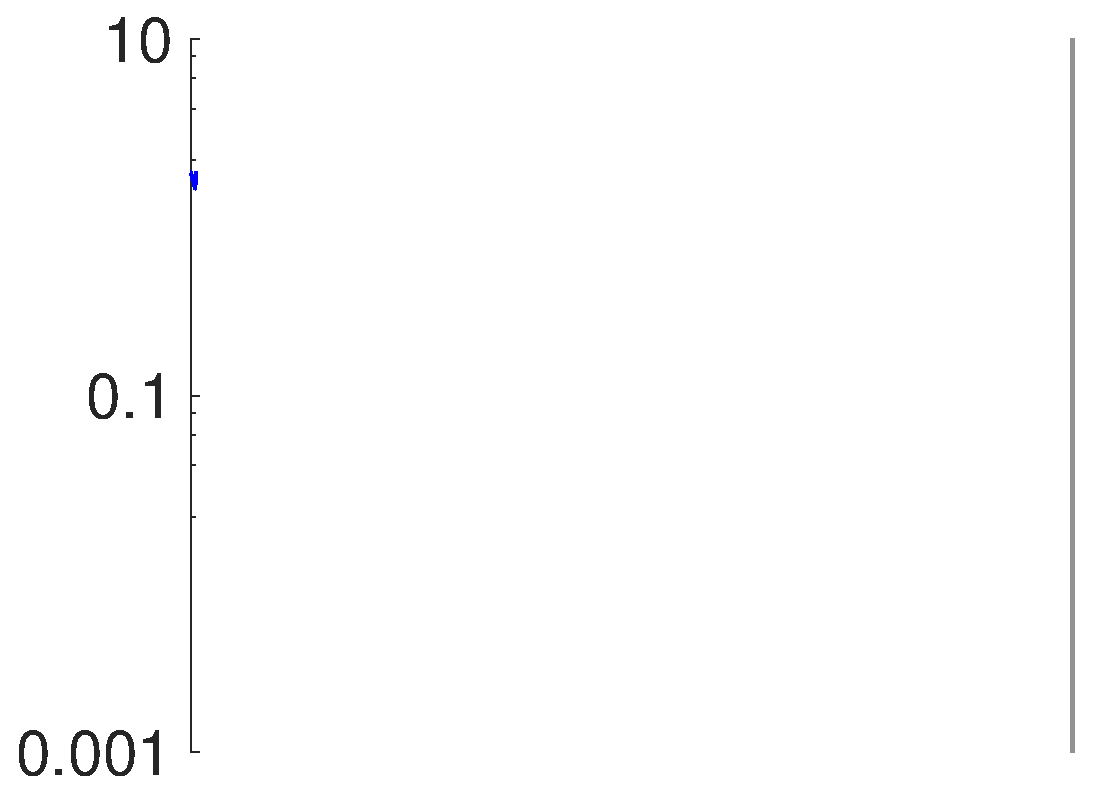
\includegraphics[trim=0cm 0cm 0cm 0cm,clip=true,height=0.15\linewidth,width=.4\linewidth]{Figures/Fig_T5/MATLAB/ST_T2_Seg3_Var_MSE.eps}
        \hspace{1.5em}
        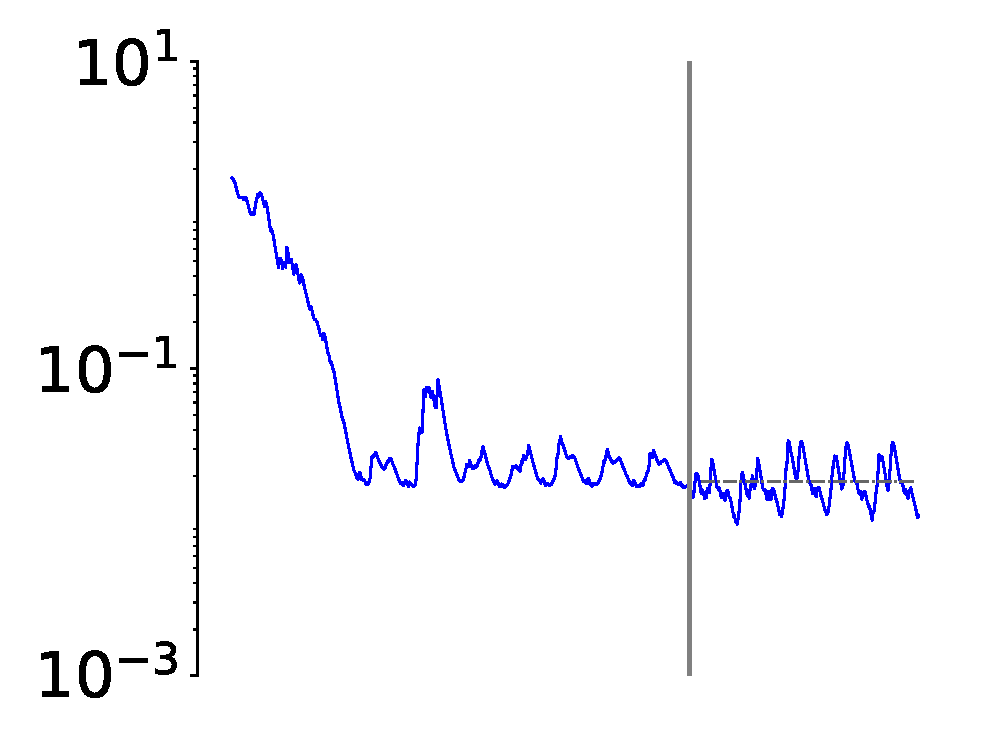
\includegraphics[trim=0cm 0cm 0cm 0cm,clip=true,clip=true,height=0.15\linewidth,width=.45\linewidth]{Figures/Fig_T5/ImprovP/ST_T2_Seg3_Var_MSE.eps}
    
    \end{subfigure}
        
    
        
        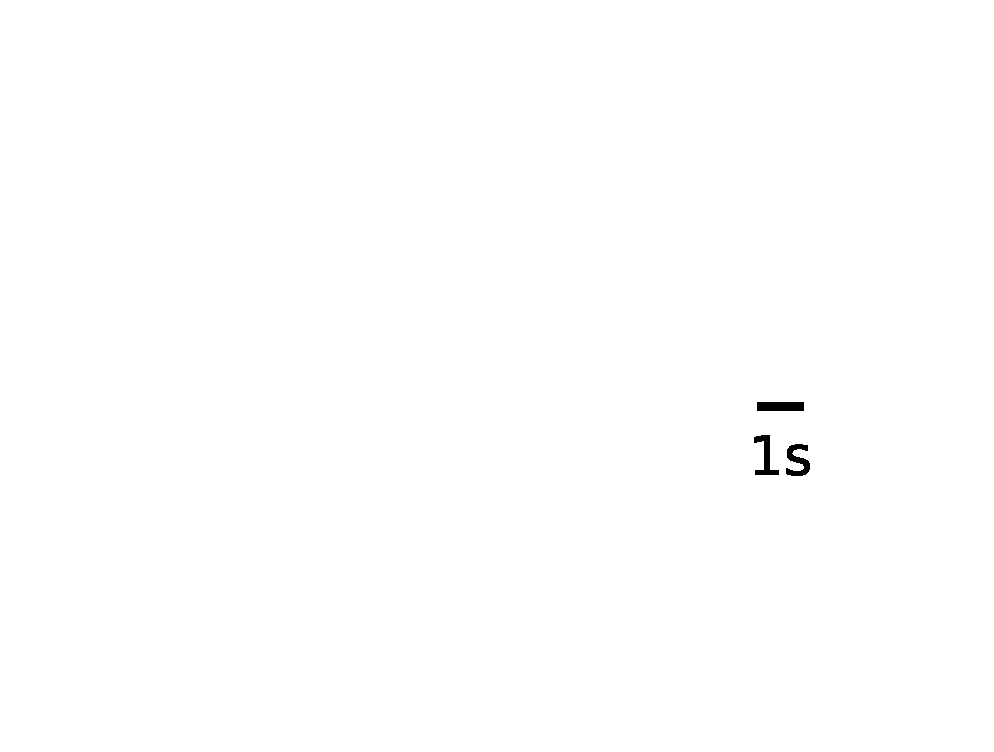
\includegraphics[trim=2cm 6cm 2cm 6cm, clip=true,height=0.05\linewidth,width=.4\linewidth]{Figures/Fig_T1/Python/ST_T1_Scale.eps}
        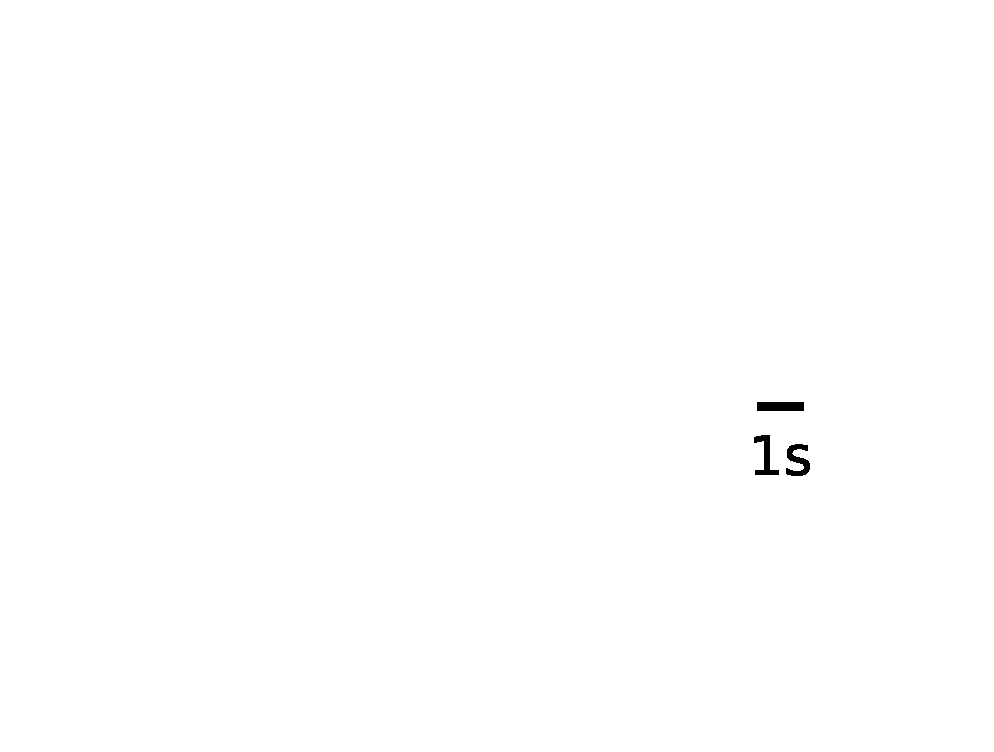
\includegraphics[trim=2cm 4cm 2cm 6cm, clip=true,height=0.05\linewidth,width=.45\linewidth]{Figures/Fig_T1/Python/ST_T1_Scale.eps}



\caption{Robustness of the SUPERTREX model on a Task 2 variant. The performance of the original scripts (left column) and modified Python re-implementation (right column) is tested for the SUPERTREX learning algorithm on a variant of Task 2 with increased number of arm segments (lengths: 1.8, 1.2, 0.6). The top panel shows the target trajectory (red) with the trajectory generated by the algorithm (blue) throughout the test phase. The next three rows show the time-series (blue) generated by the model (joint angles ($\theta_i$), in this case). The fourth row shows the progression of the norm of the weight matrix ($W_1$ in purple; $W_2$, in green). The bottom row shows the distance from target metric (blue) over the simulation, using the log scale for the y axis. The horizontal grey line, in the test phase, indicates the deviation metric. The grey vertical line marks the separation of the training and testing phase. Using the MATLAB scripts, the readout weights increase uncontrollably rendering the model unable to learn. The Python re-implementation, using a compensation factor to harness the weight update, is able to learn and converge to produce the target time-series.}
\label{Fig:Comparison_Task2_Seg3}

\end{figure}

